\documentclass[pdflatex,compress]{beamer}

%\usetheme[dark,framenumber,totalframenumber]{ElektroITK}
\usetheme[darktitle,framenumber,totalframenumber]{ElektroITK}

\usepackage[utf8]{inputenc}
\usepackage[T1]{fontenc}
\usepackage{lmodern}
\usepackage[bahasai]{babel}
\usepackage{amsmath}
\usepackage{amsfonts}
\usepackage{amssymb}
\usepackage{graphicx}
\usepackage{multicol}
\usepackage{lipsum}
\usefonttheme[onlymath]{serif}

\newcommand*{\Scale}[2][4]{\scalebox{#1}{$#2$}}%

\title{METODE NUMERIK}
\subtitle{Interpolasi dan Regresi}

\author{Mifta Nur Farid}

\begin{document}

\maketitle

\section{Pengantar}

\begin{frame}
	\frametitle{Pengantar}
	\begin{itemize}
		\item Misalkan diketahui tabel hasil pembacaan suhu dari suatu reaksi kimia sebagai berikut
		\begin{center}
			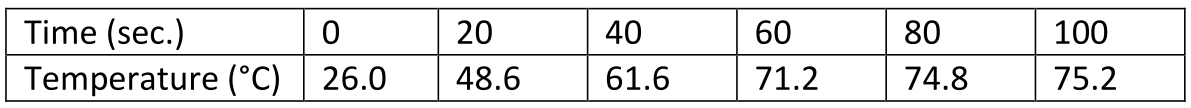
\includegraphics[width=0.8\linewidth]{img/img01}
		\end{center}
		\item Kemudian linear plot dari data di atas adalah:
		\begin{center}
			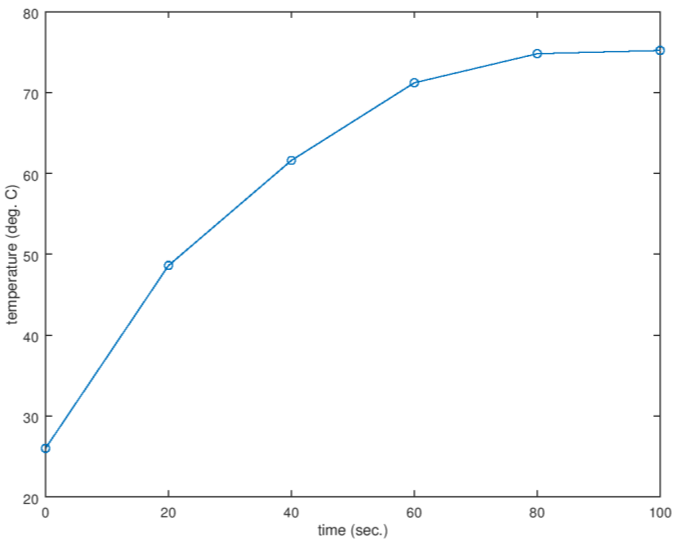
\includegraphics[width=0.5\linewidth]{img/img02}
		\end{center}
	\end{itemize}
\end{frame}

\begin{frame}{Pengantar}
	\begin{itemize}
		\item Berdasarkan data tersebut, jika kita memerlukan suhu reaksi saat detik ke 50, bagaimana cara kita memperoleh data tersebut?
		\item Cara yang dapat kita lakukan adalah melakukan \textbf{interpolasi}.
		\item Kita akan mempelajari interpolasi dan regresi.
	\end{itemize}
\end{frame}

\begin{frame}
	\frametitle{Sub-CPMK}
	\textbf{Sub Capaian Pembelajaran Mata Kuliah (Sub-CPMK):} Mahasiswa mampu melakukan interpolasi dan regresi
\end{frame}

\begin{frame}
	\frametitle{Bahan Kajian}
	\begin{enumerate}
		\item Interpolasi linear;
		\item Interpolasi Lagrange
		\item Interpolasi Newton
		\item Regresi linier;
	\end{enumerate}
\end{frame}

\section{Interpolasi Linear}

\begin{frame}
	\frametitle{Interpolasi Linear}
	\begin{itemize}
		\item Misalkan diketahui tabel hasil pembacaan suhu dari suatu reaksi kimia sebagai berikut
		\begin{center}
			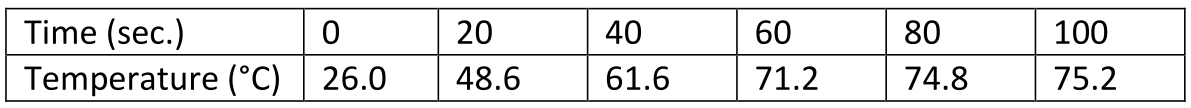
\includegraphics[width=0.8\linewidth]{img/img01}
		\end{center}
		\item Kemudian linear plot dari data di atas adalah:
		\begin{center}
			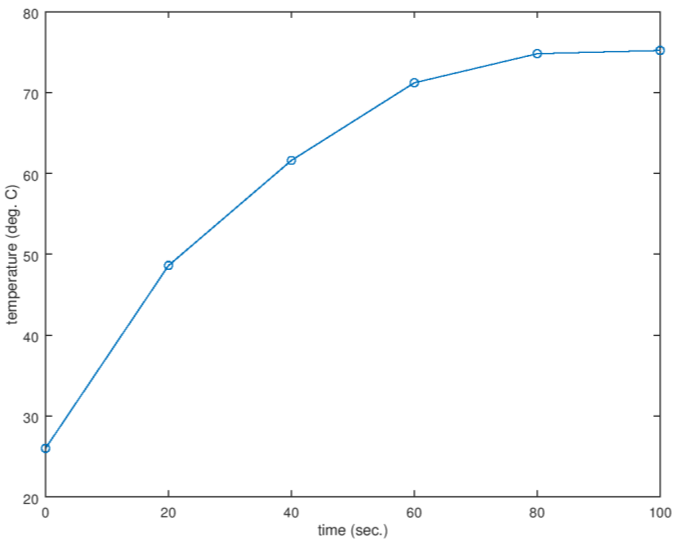
\includegraphics[width=0.5\linewidth]{img/img02}
		\end{center}
	\end{itemize}
\end{frame}

\begin{frame}{Interpolasi Linear}
	\begin{itemize}
		\item Berdasarkan data tersebut, jika kita memerlukan suhu reaksi saat detik ke 50, bagaimana cara kita memperoleh data tersebut?
		\item Metode yang paling mudah adalah dengan menggunakan metode \textbf{interpolasi linear}.
	\end{itemize}
\end{frame}

\begin{frame}{Interpolasi Linear}
	\begin{itemize}
		\item Mengambil bagian dari kurva yang menghubungkan 2 titik yang telah diketahui, $ (x_1, y_1) $ dan $ (x_2, y_2) $
		\begin{center}
			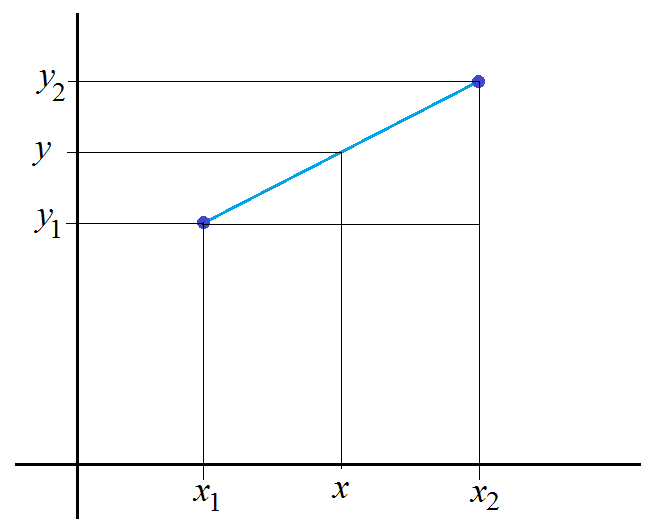
\includegraphics[width=0.5\linewidth]{img/img03}
		\end{center}
		\item Dari kasus di atas maka $ (x_1, y_1) $ dan $ (x_2, y_2) $ adalah $ (40, 61.6) $ dan $ (60, 71.2) $
	\end{itemize}
\end{frame}

\begin{frame}{Interpolasi Linear}
	\begin{itemize}
		\item Karena gradient dari kurva tsb adalah sama
		\begin{center}
			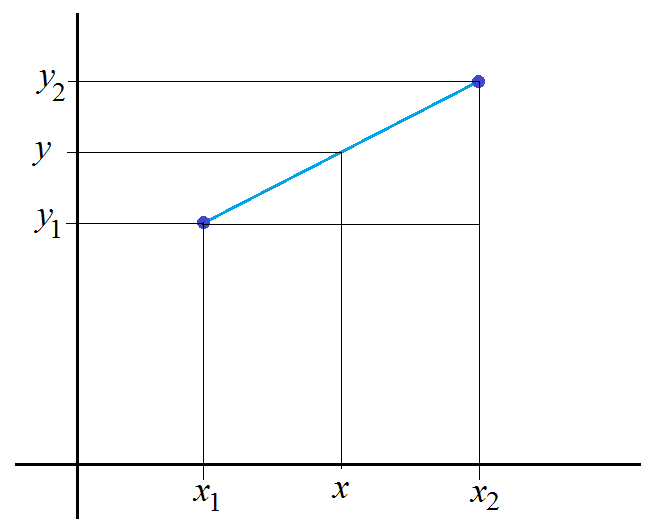
\includegraphics[width=0.4\linewidth]{img/img03}
		\end{center}
		maka
		\begin{equation*}
			\frac{y - y_1}{x - x_1} = \frac{y_2 - y_1}{x_2 - x_1}
		\end{equation*}
		\item Kita dapatkan
		\begin{equation*}
			y= \frac{y_2 - y_1}{x_2 - x_1}(x - x_1) +  y_1
		\end{equation*}
	\end{itemize}
\end{frame}

\begin{frame}{Interpolasi Linear}
	\begin{itemize}
		\item Sehingga dari kasus di atas, maka
		\begin{align*}
			y &= \frac{y_2 - y_1}{x_2 - x_1}(x - x_1) +  y_1 \\
			&= \frac{71.2 - 61.6}{60 - 40}(50 - 40) +  61.6 \\
			&= 66.4^\circ \text{C}
		\end{align*}
	\end{itemize}
\end{frame}

\begin{frame}{Interpolasi Linear}
	\begin{itemize}
		\item Kekurangan metode interpolasi linear adalah titik-titik lain selain dua titik yang berdekatan dibaikan.
		\item Artinya, trend dari kurva keseluruhan dataset tidak dihitung sehingga titik interpolasi tidak secara akurat terletak pada kurva itu.
	\end{itemize}
\end{frame}

\section{Interpolasi Lagrange}

\begin{frame}
	\frametitle{Interpolasi Lagrange}
	\begin{itemize}
		\item Metode interpolasi Lagrange didasari oleh pembuatan polinomial derajat $ n $.
		\item Derajatnya bergantung pada banyaknya titik yang ada di dalam dataset, yaitu sebanyak $ n + 1 $ titik.
		\item Contoh: untuk polinomial derajat 3 (kubik), $ n = 3 $, maka 4 titik yang dibutuhkan.
	\end{itemize}
\end{frame}

\begin{frame}{Interpolasi Lagrange}
	\begin{itemize}
		\item Sehingga
		\begin{equation*}
			y(x) = y_1 l_1(x) + y_2 l_2(x) + y_3 l_3(x) + y_4 l_4(x)
		\end{equation*}
		yang mana
		\begin{align*}
			l_1(x) &= \frac{(x-x_2)(x-x_3)(x-x_4)}{(x_1-x_2)(x_1-x_3)(x_1-x_4)} \\
			l_2(x) &= \frac{(x-x_1)(x-x_3)(x-x_4)}{(x_2-x_1)(x_2-x_3)(x_2-x_4)} \\
			l_3(x) &= \frac{(x-x_1)(x-x_2)(x-x_4)}{(x_3-x_1)(x_3-x_2)(x_3-x_4)} \\
			l_4(x) &= \frac{(x-x_1)(x-x_2)(x-x_3)}{(x_4-x_1)(x_4-x_2)(x_4-x_3)}
		\end{align*}
	\end{itemize}
\end{frame}

\begin{frame}{Interpolasi Lagrange}
	\begin{itemize}
		\item atau
		\begin{equation*}
			l_i(x) = \prod\limits_{j = 1;~j \neq i}^{n+1} \frac{(x - x_j)}{x_i - x_j}
		\end{equation*}
		sehingga persamaan dari metode interpolasi Lagrange
		\begin{equation*}
			y(x) = \sum\limits_{i=1}^{n+1}y_i \left( \prod\limits_{j = 1;~j \neq i}^{n+1} \frac{(x - x_j)}{x_i - x_j} \right)
		\end{equation*}
		\item Kita coba selesaikan contoh sebelumnya dengan metode interpolasi Lagrange kemudian bandingkan dengan hasil interpolasi linear.
	\end{itemize}
\end{frame}

\section{Interpolasi Newton}

\begin{frame}
	\frametitle{Interpolasi Newton}
	\begin{itemize}
		\item Menggunakan polinomial Newton
		\begin{align*}
			y(x) =& a_0 + (x - x_1)a_1 + (x - x_1)(x - x_2)a_2 \\
			&+ \cdots + (x - x_1)(x - x_2) \dots (x - x_n)a_n
		\end{align*}
		\item Terdapat 2 langkah:
		\begin{enumerate}
			\item Membuat tabel beda terbagi (\textit{divided differences})
			\item Substitusi nilai $ x $ yang diketahui ke dalam persamaan polinomial untuk mendapatkan nilai $ y $ yang diinterpolasi.
		\end{enumerate}
	\end{itemize}
\end{frame}

\begin{frame}{Interpolasi Newton}
	\begin{itemize}
		\item Tabel beda terbagi
		\begin{center}
			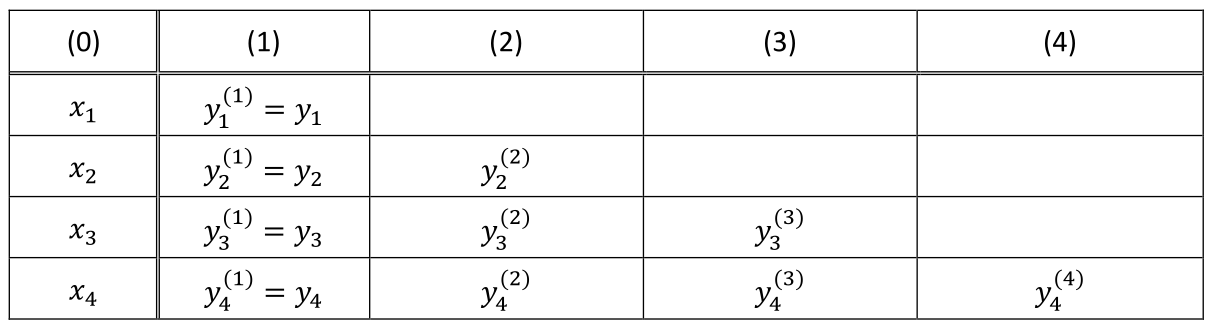
\includegraphics[width=\linewidth]{img/img04}
		\end{center}
		\item Untuk kolom ke (2)
		\begin{align*}
			y_i^{(2)} = \frac{y_i^{(1)} - y_1^{(1)}}{x_i - x_1},~i = 2,3,4
		\end{align*}
	\end{itemize}
\end{frame}

\begin{frame}{Interpolasi Newton}
	\begin{itemize}
		\item Untuk kolom ke (3)
		\begin{align*}
			y_i^{(3)} = \frac{y_i^{(2)} - y_2^{(2)}}{x_i - x_2},~i = 3,4
		\end{align*}
		\item Untuk kolom ke (4)
		\begin{align*}
			y_4^{(4)} = \frac{y_4^{(3)} - y_3^{(3)}}{x_4 - x_3}
		\end{align*}
	\end{itemize}
\end{frame}

\begin{frame}{Interpolasi Newton}
	\begin{itemize}
		\item sehingga persamaan umumnya
		\begin{align*}
			y_i^{(j+1)} = \frac{y_i^{(j)} - y_j^{(j)}}{x_i - x_j},~j=1,\dots,n\text{ dan } i = j+1,\dots,n+1
		\end{align*}
		yang mana $ y_1^{(1)} = y_1 $ dan $ y_2^{(1)} = y_2 $ dan seterusnya
	\end{itemize}
\end{frame}

\begin{frame}{Interpolasi Newton}
	\begin{itemize}
		\item koefisien polinomial adalah nilai diagonal utama dari tabel beda terbagi
		\begin{equation*}
			a_0 = y_1^{(1)},~a_1 = y_2^{(2)},~a_2 = y_3^{(3)},\dots,~a_n = y_n+1^{(n+1)}
		\end{equation*}
		\begin{center}
			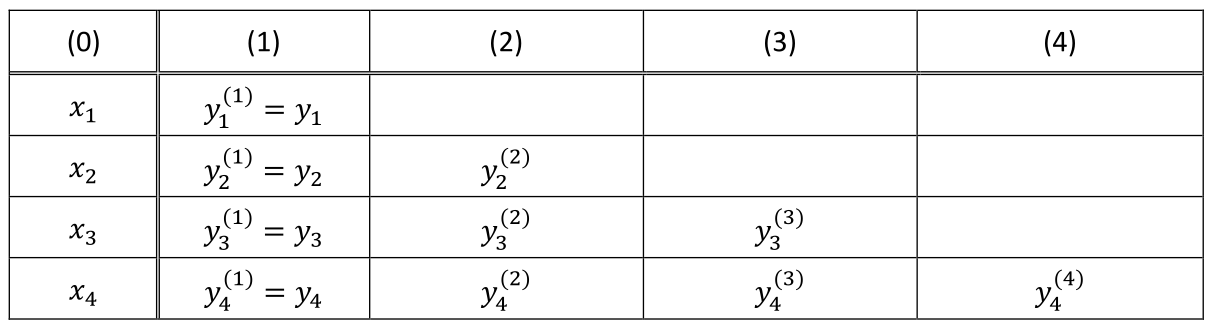
\includegraphics[width=\linewidth]{img/img04}
		\end{center}
	\end{itemize}
\end{frame}

\begin{frame}{Interpolasi Newton}
	\begin{itemize}
		\item sehingga persamaan dari metode interpolasi Newton adalah
		\begin{equation*}
			y(x) = a_0 + \sum\limits_{i = 1}^{n} \left[ \prod\limits_{j = 1}^{i} (x - x_j) \right] a_i
		\end{equation*}
		atau
		\begin{equation*}
			y(x) = y_1^{(1)} + \sum\limits_{i = 1}^{n} \left[ \prod\limits_{j = 1}^{i} (x - x_j) \right] y_{i+1}^{(i+1)}
		\end{equation*}
		\item Kita coba selesaikan contoh sebelumnya dengan metode interpolasi Newton kemudian bandingkan dengan hasil interpolasi Lagrange dan interpolasi linear.
	\end{itemize}
\end{frame}

\section{Regresi Linear}

\begin{frame}
	\frametitle{Regresi Linear}
	\centering
	\textbf{Pertemuan Berikutnya}
\end{frame}

\end{document}
